\documentclass[10pt,twocolumn,letterpaper]{article}

\usepackage{cvpr}
\usepackage{times}
\usepackage{epsfig}
\usepackage{graphicx}
\usepackage{amsmath}
\usepackage{amssymb}

% Include other packages here, before hyperref.
\usepackage[pagebackref=true,breaklinks=true,letterpaper=true,colorlinks,bookmarks=false]{hyperref}

% Pages are numbered in submission mode, and unnumbered in camera-ready
\ifcvprfinal\pagestyle{empty}\fi
\begin{document}

%%%%%%%%% TITLE
\title{Otsu's Method: Classic vs New Technique}

\author{Konstantinos Katergaris\\
Arizona State University\\
1151 S Forest Ave, Tempe, AZ\\
{\tt\small kkaterga@asu.edu}}

%\thispagestyle{empty}

\maketitle
\begin{abstract}
 This report discusses Otsu's method, a classic thresholding algorithm that separates an image into foreground and background. The report highlights the implementation of this algorithm, its multi-threshold version, as well as a new approach \cite{Huang2014}. Additionally, it presents results one real world example and compares each output.
\end{abstract}
\section{Overveiw}
\subsection{Otsu's method}
Otsu's method\cite{4310076} is a technique that determines a single threshold value by maximizing the between-class variance, effectively separating the image into foreground and background. The process begins with creating a histogram that maps pixel intensities from 0 to 255 in an 8-bit image. This histogram is then normalized. For each potential threshold, a cumulative sum is calculated, representing the probability of an object or background, while the cumulative mean is computed to average the pixel intensities up to that threshold. Next, the global mean pixel intensity is calculated. Additionally, the between-class variance is computed for each possible threshold, which measures how distinct the foreground and background intensities are based on the cumulative sums and means. Finally, the threshold is calculated by maximizing the  between-class that best separates the foreground from the background.
\subsection{ Multi-Threshold Otsu's}
This is an extension of Otsu's method \cite{4310076}, which iteratively applies the algorithm to enable the separation of multiple objects from an image. The process begins by calculating the first threshold and applying it to the image. The method is then repeated, recalculating and applying additional thresholds until the desired number of classes is achieved.
\subsection{Valleys Otsu's}
This is a modification of multi-thresholding \cite{Huang2014} that identifies local minima in the histogram and uses them to help segment the image. The histogram is first divided into smaller bins to simplify the process of finding local minima. Afterward, the local minima are calculated, and Otsu's method is applied to each of these minima to identify the thresholds for the different objects in the image. 

\section{Implementation}
All these methods were implemented in Python. The NumPy library was used to handle all mathematical operations, translating mathematical notation into code. Furthermore, an edge case was added when calculating the between-class variance: if the image were to be divided by zero, meaning that either the foreground or background did not have a pixel assigned, it would instead be divided by 1e-9. Additionally, the new valley method was implemented using \cite{george_multithreshold_otsu}and slightly modified to integrate with my original code. Detail on the implimentation can be found here:\cite{katergaris_otsu_method}

Here is the outputs produced by all three methods:
\subsection{Results}
Here is the outputs produced by all three methods:
 
\begin{figure}[h!]
    \centering
    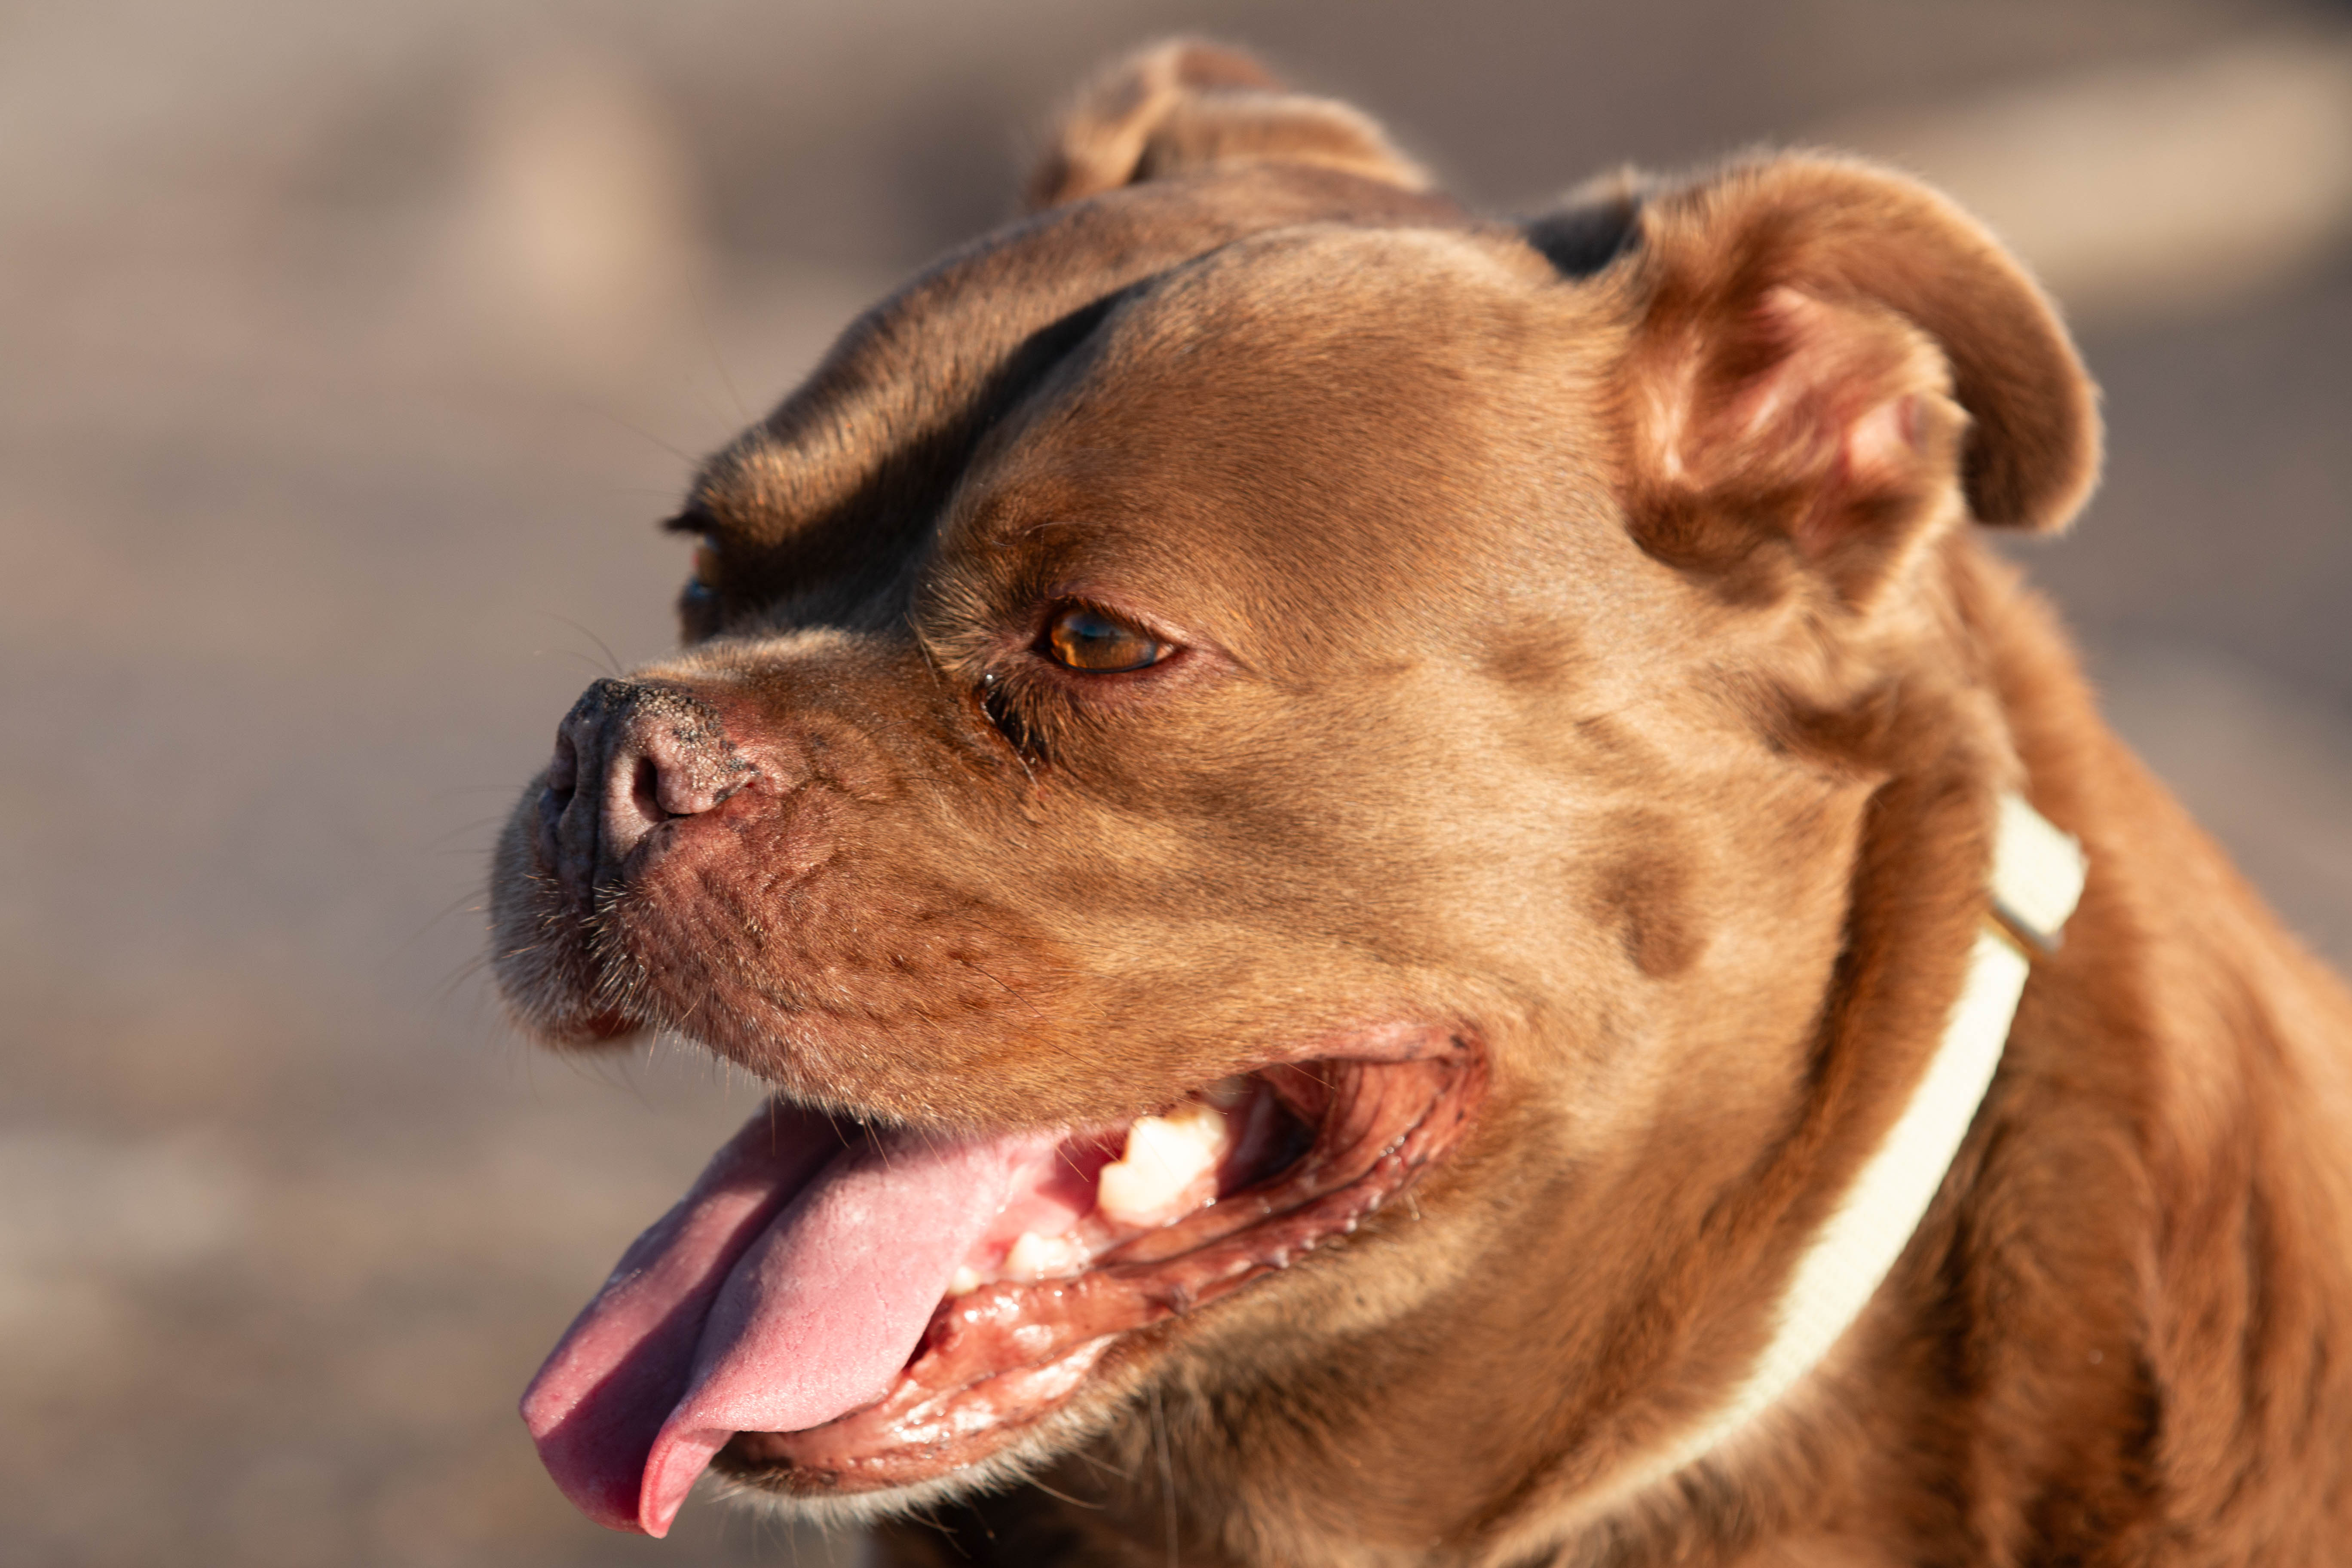
\includegraphics[width=0.8\linewidth]{port_lobos-8.jpg}
    \caption{The original image: A picture of a brown dog at the beach}
    \label{fig:JPG}
\end{figure}
\begin{figure}[h!]
    \centering
    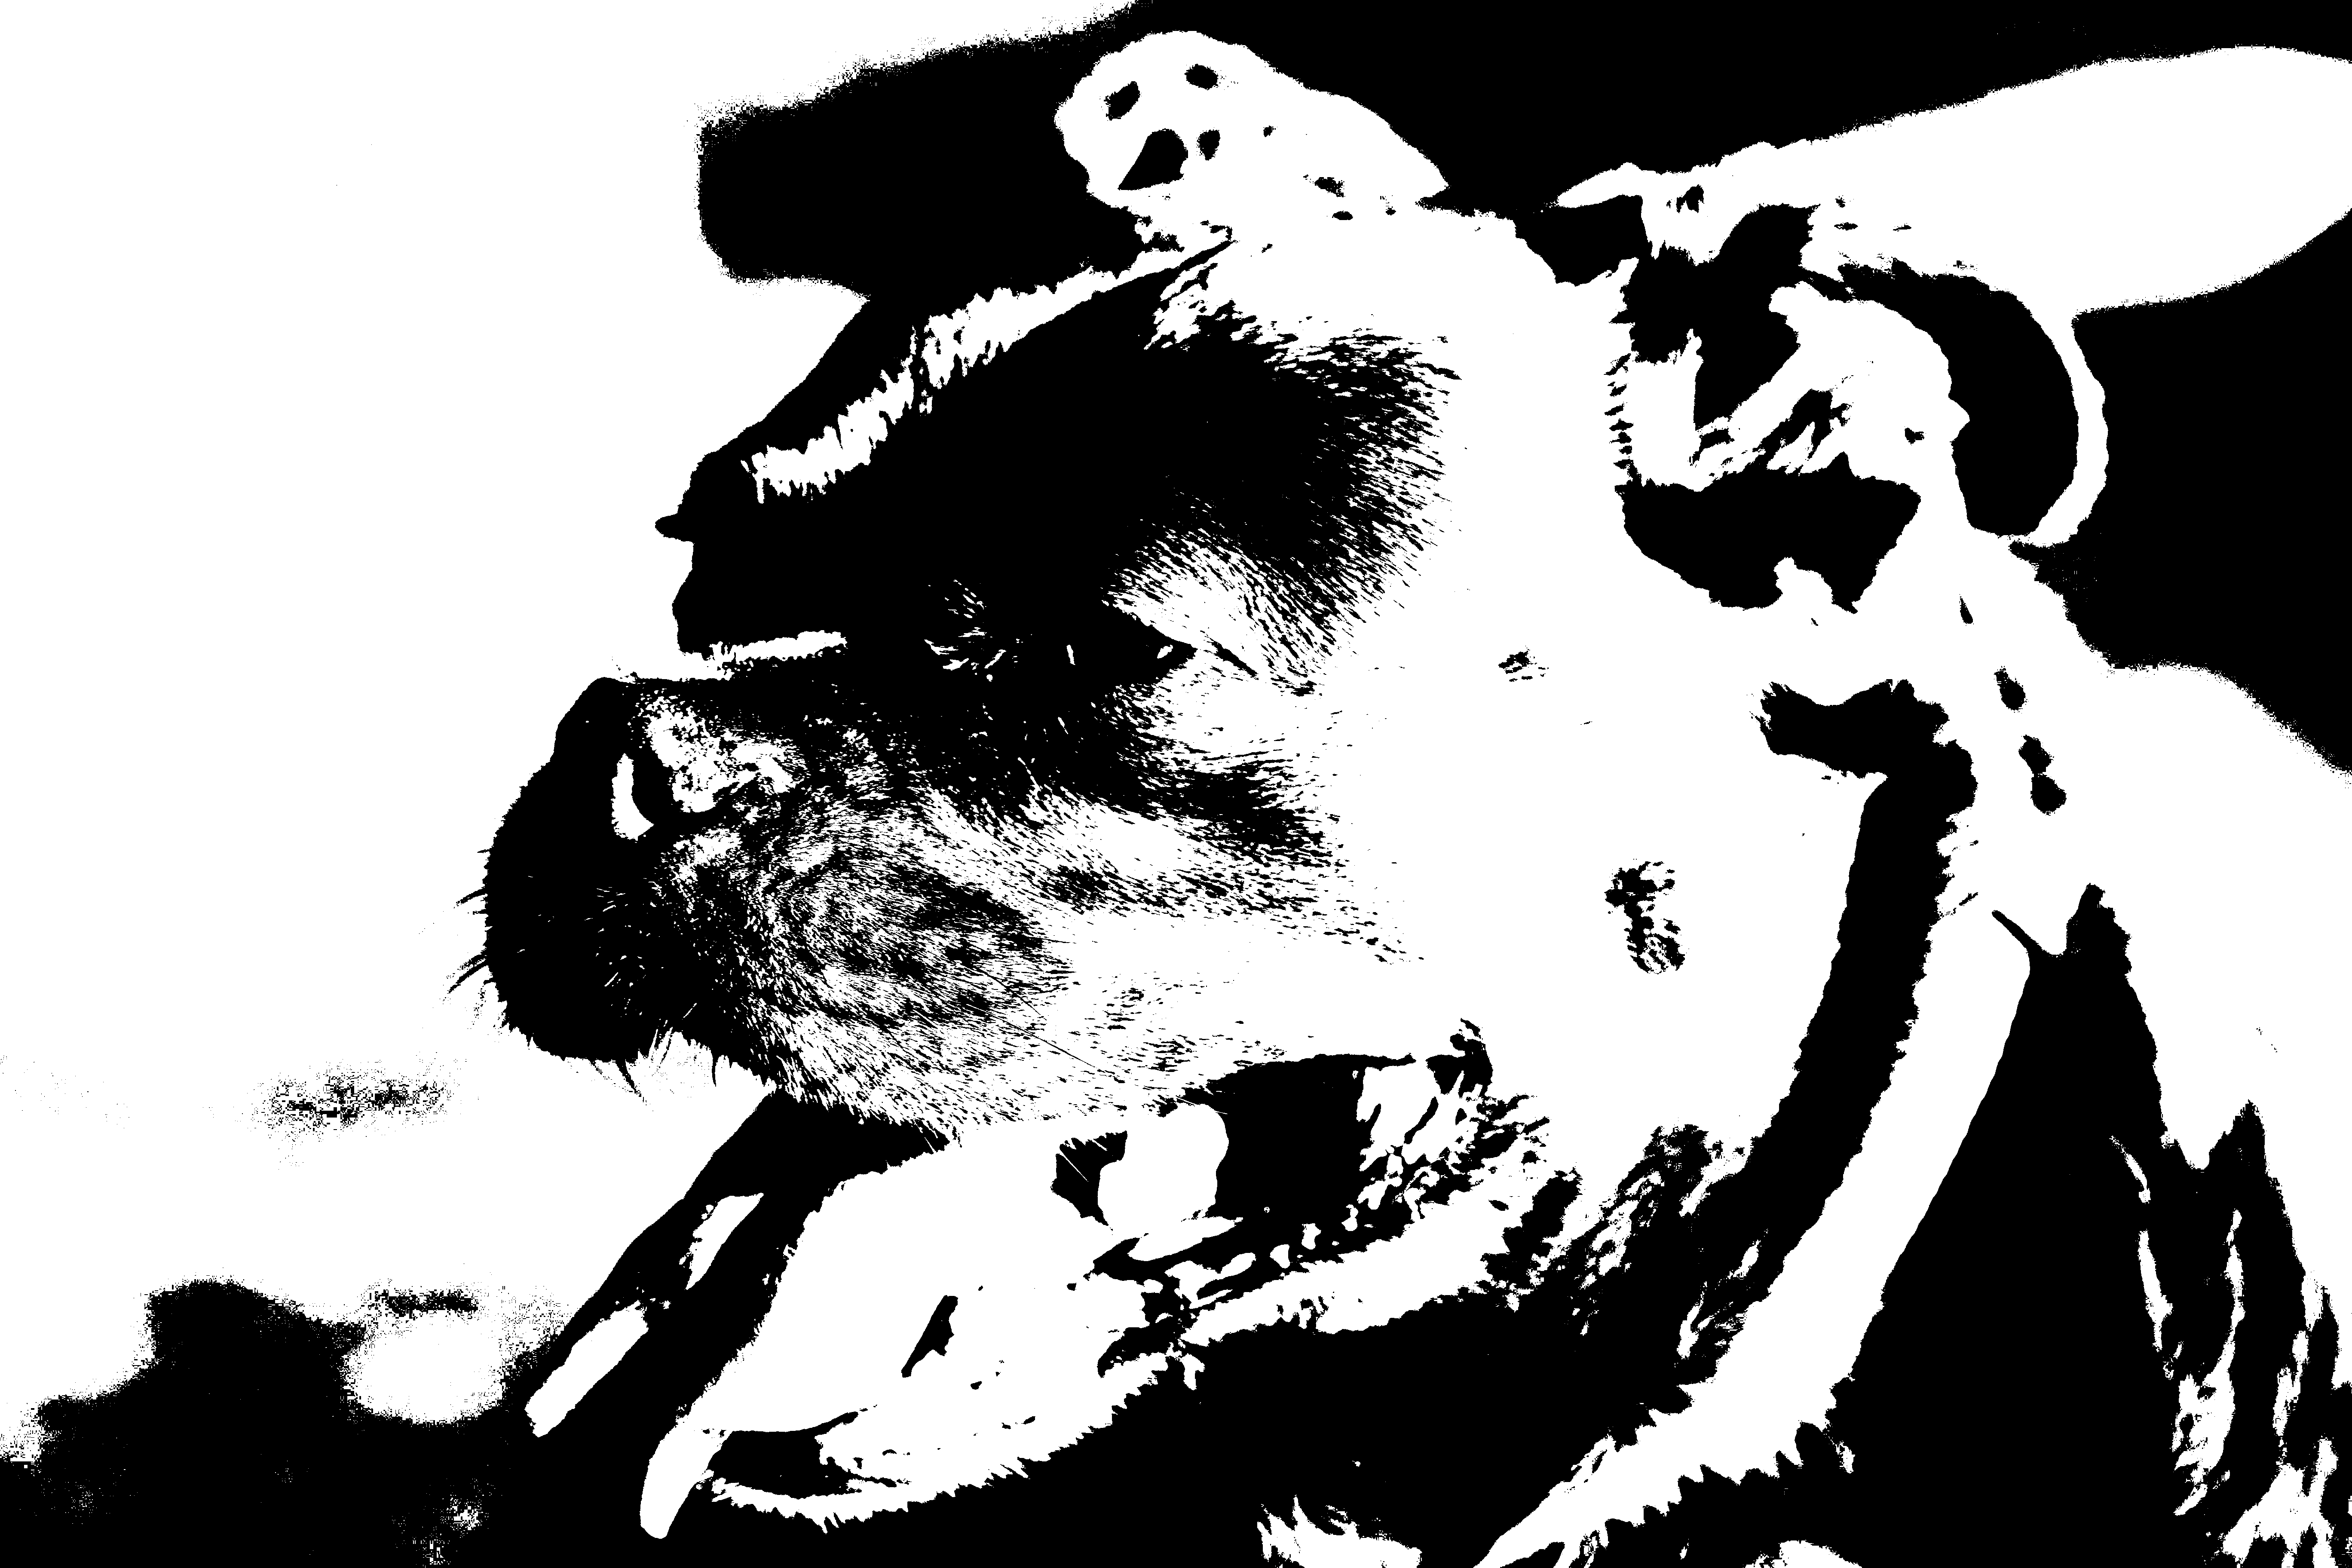
\includegraphics[width=0.8\linewidth]{otsu_threshold_image.png}
    \caption{The image produced by single-threshold Otsu's method}
    \label{fig:old}
\end{figure}
\begin{figure}[h!]
    \centering
    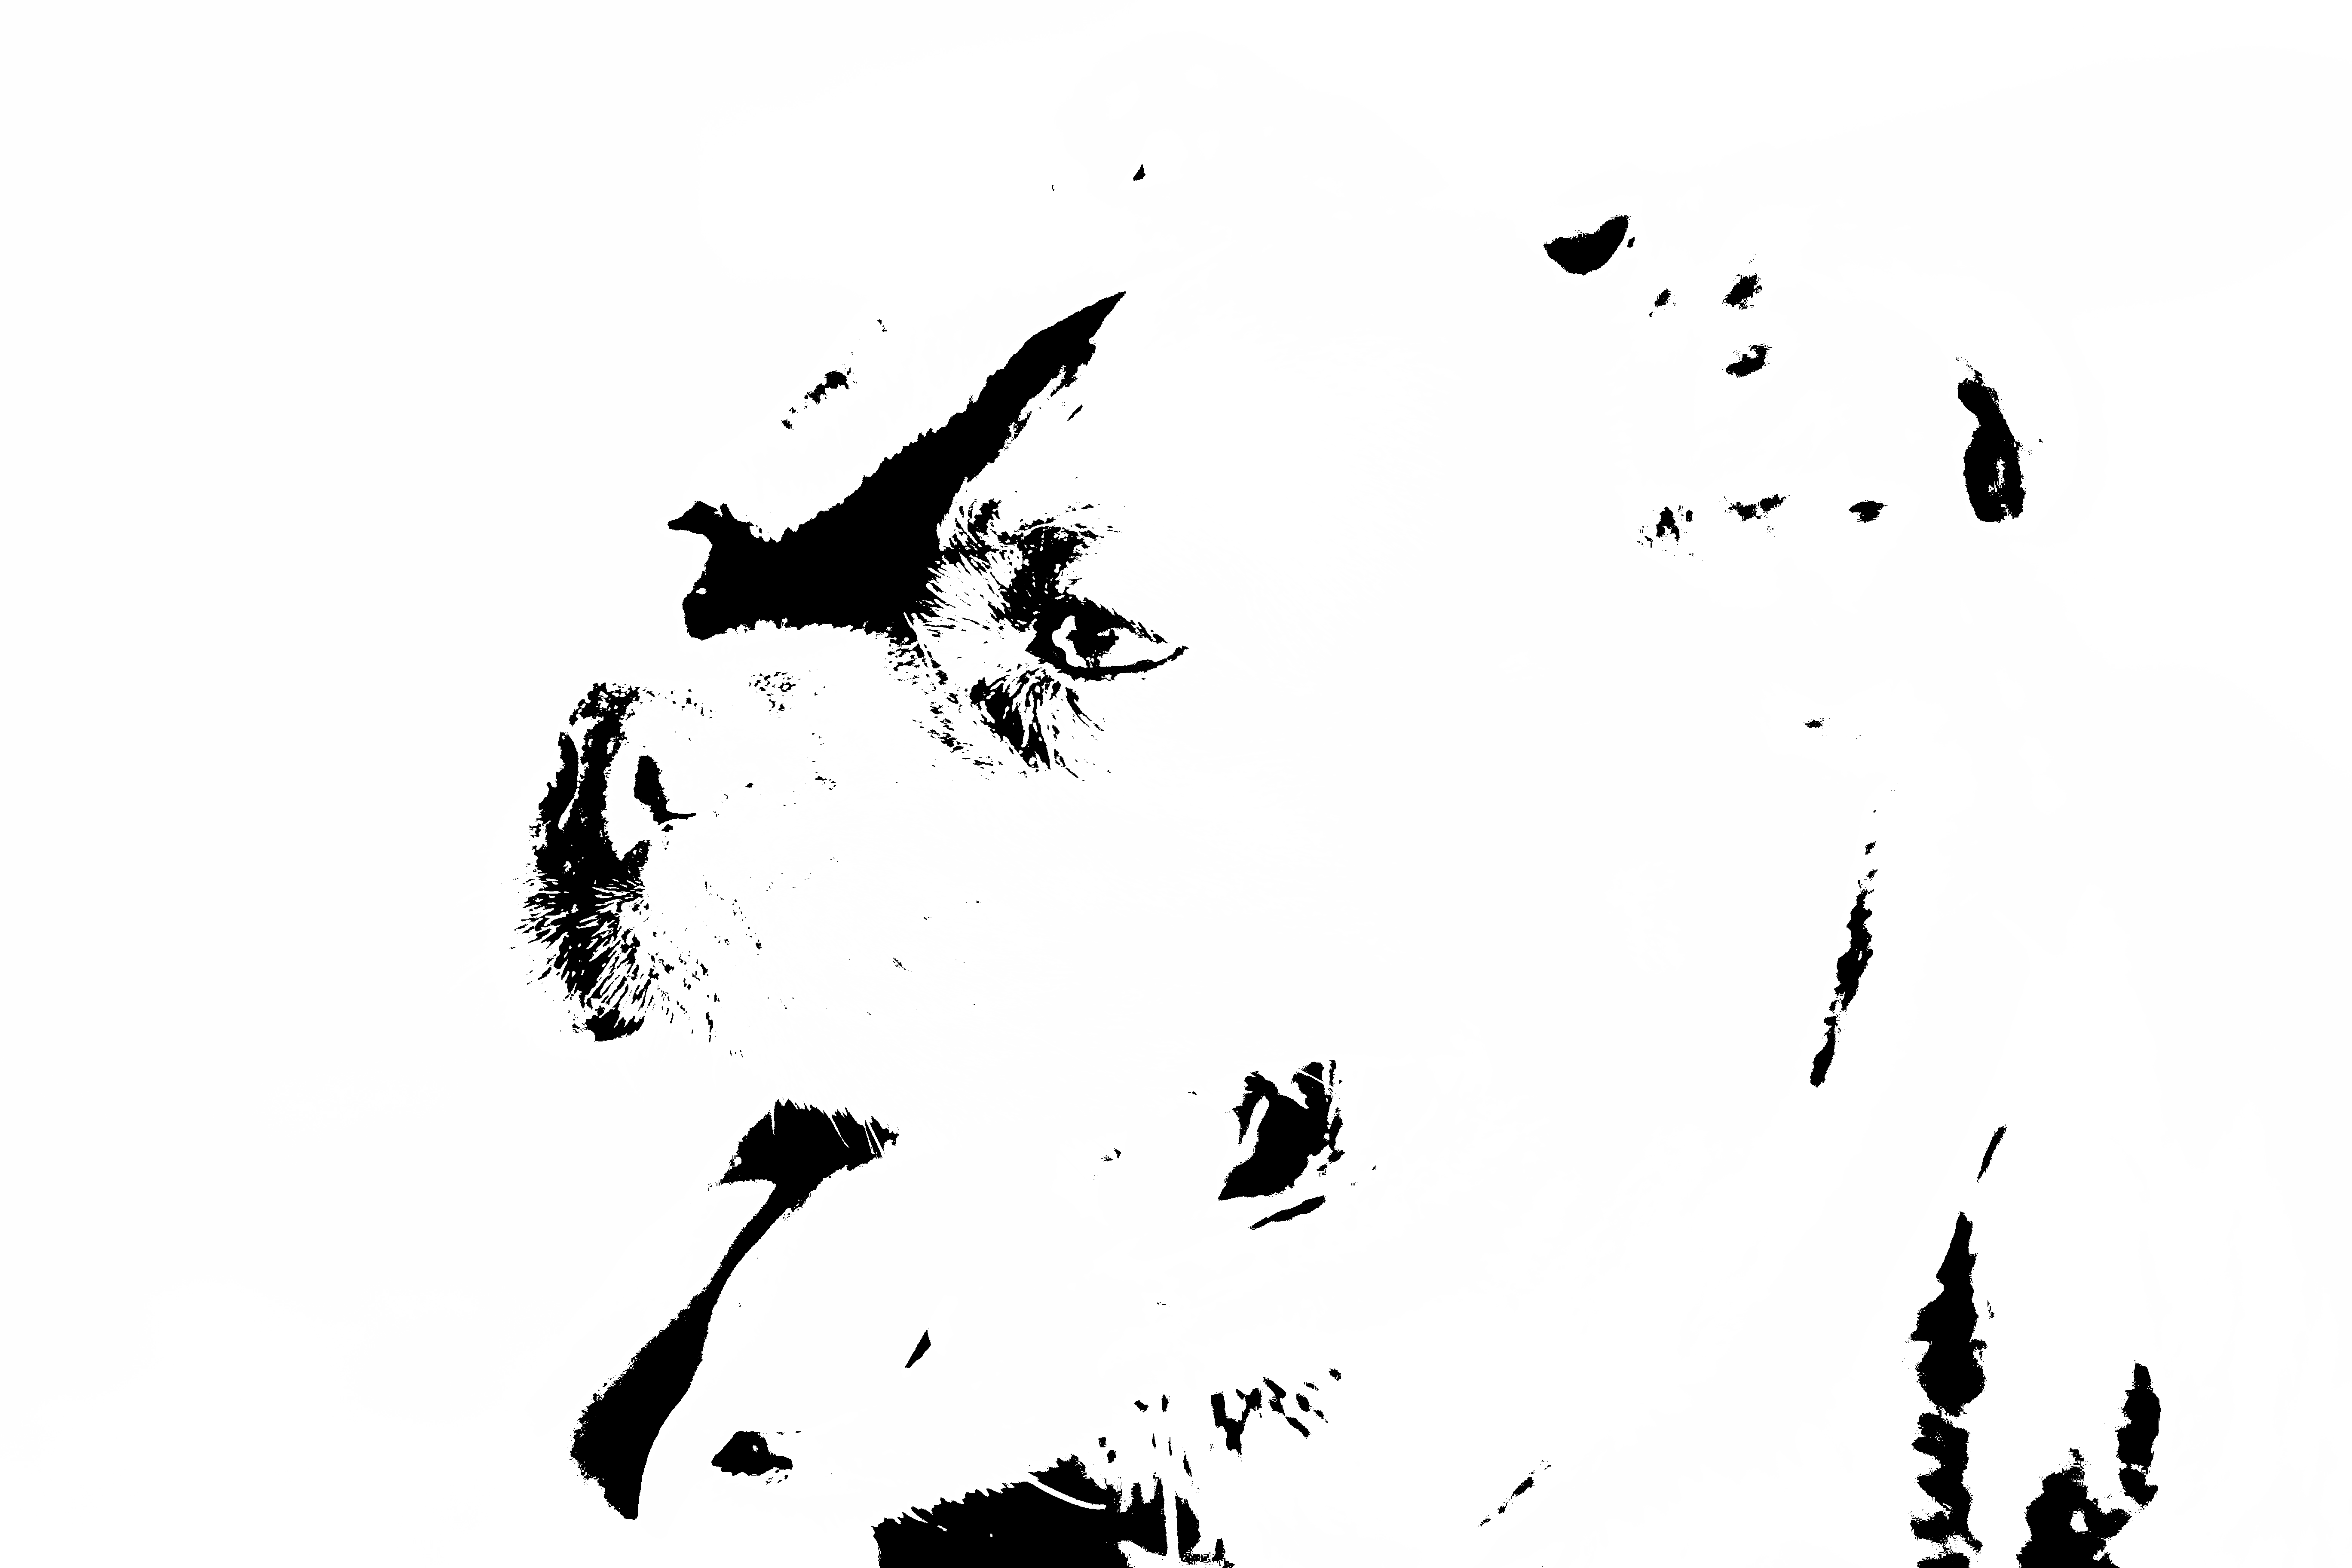
\includegraphics[width=0.8\linewidth]{multi_threshold_image.png}
    \caption{The image produced by multi-threshold Otsu's method }
    \label{fig:multi}
\end{figure}
\begin{figure}[h!]
    \centering
    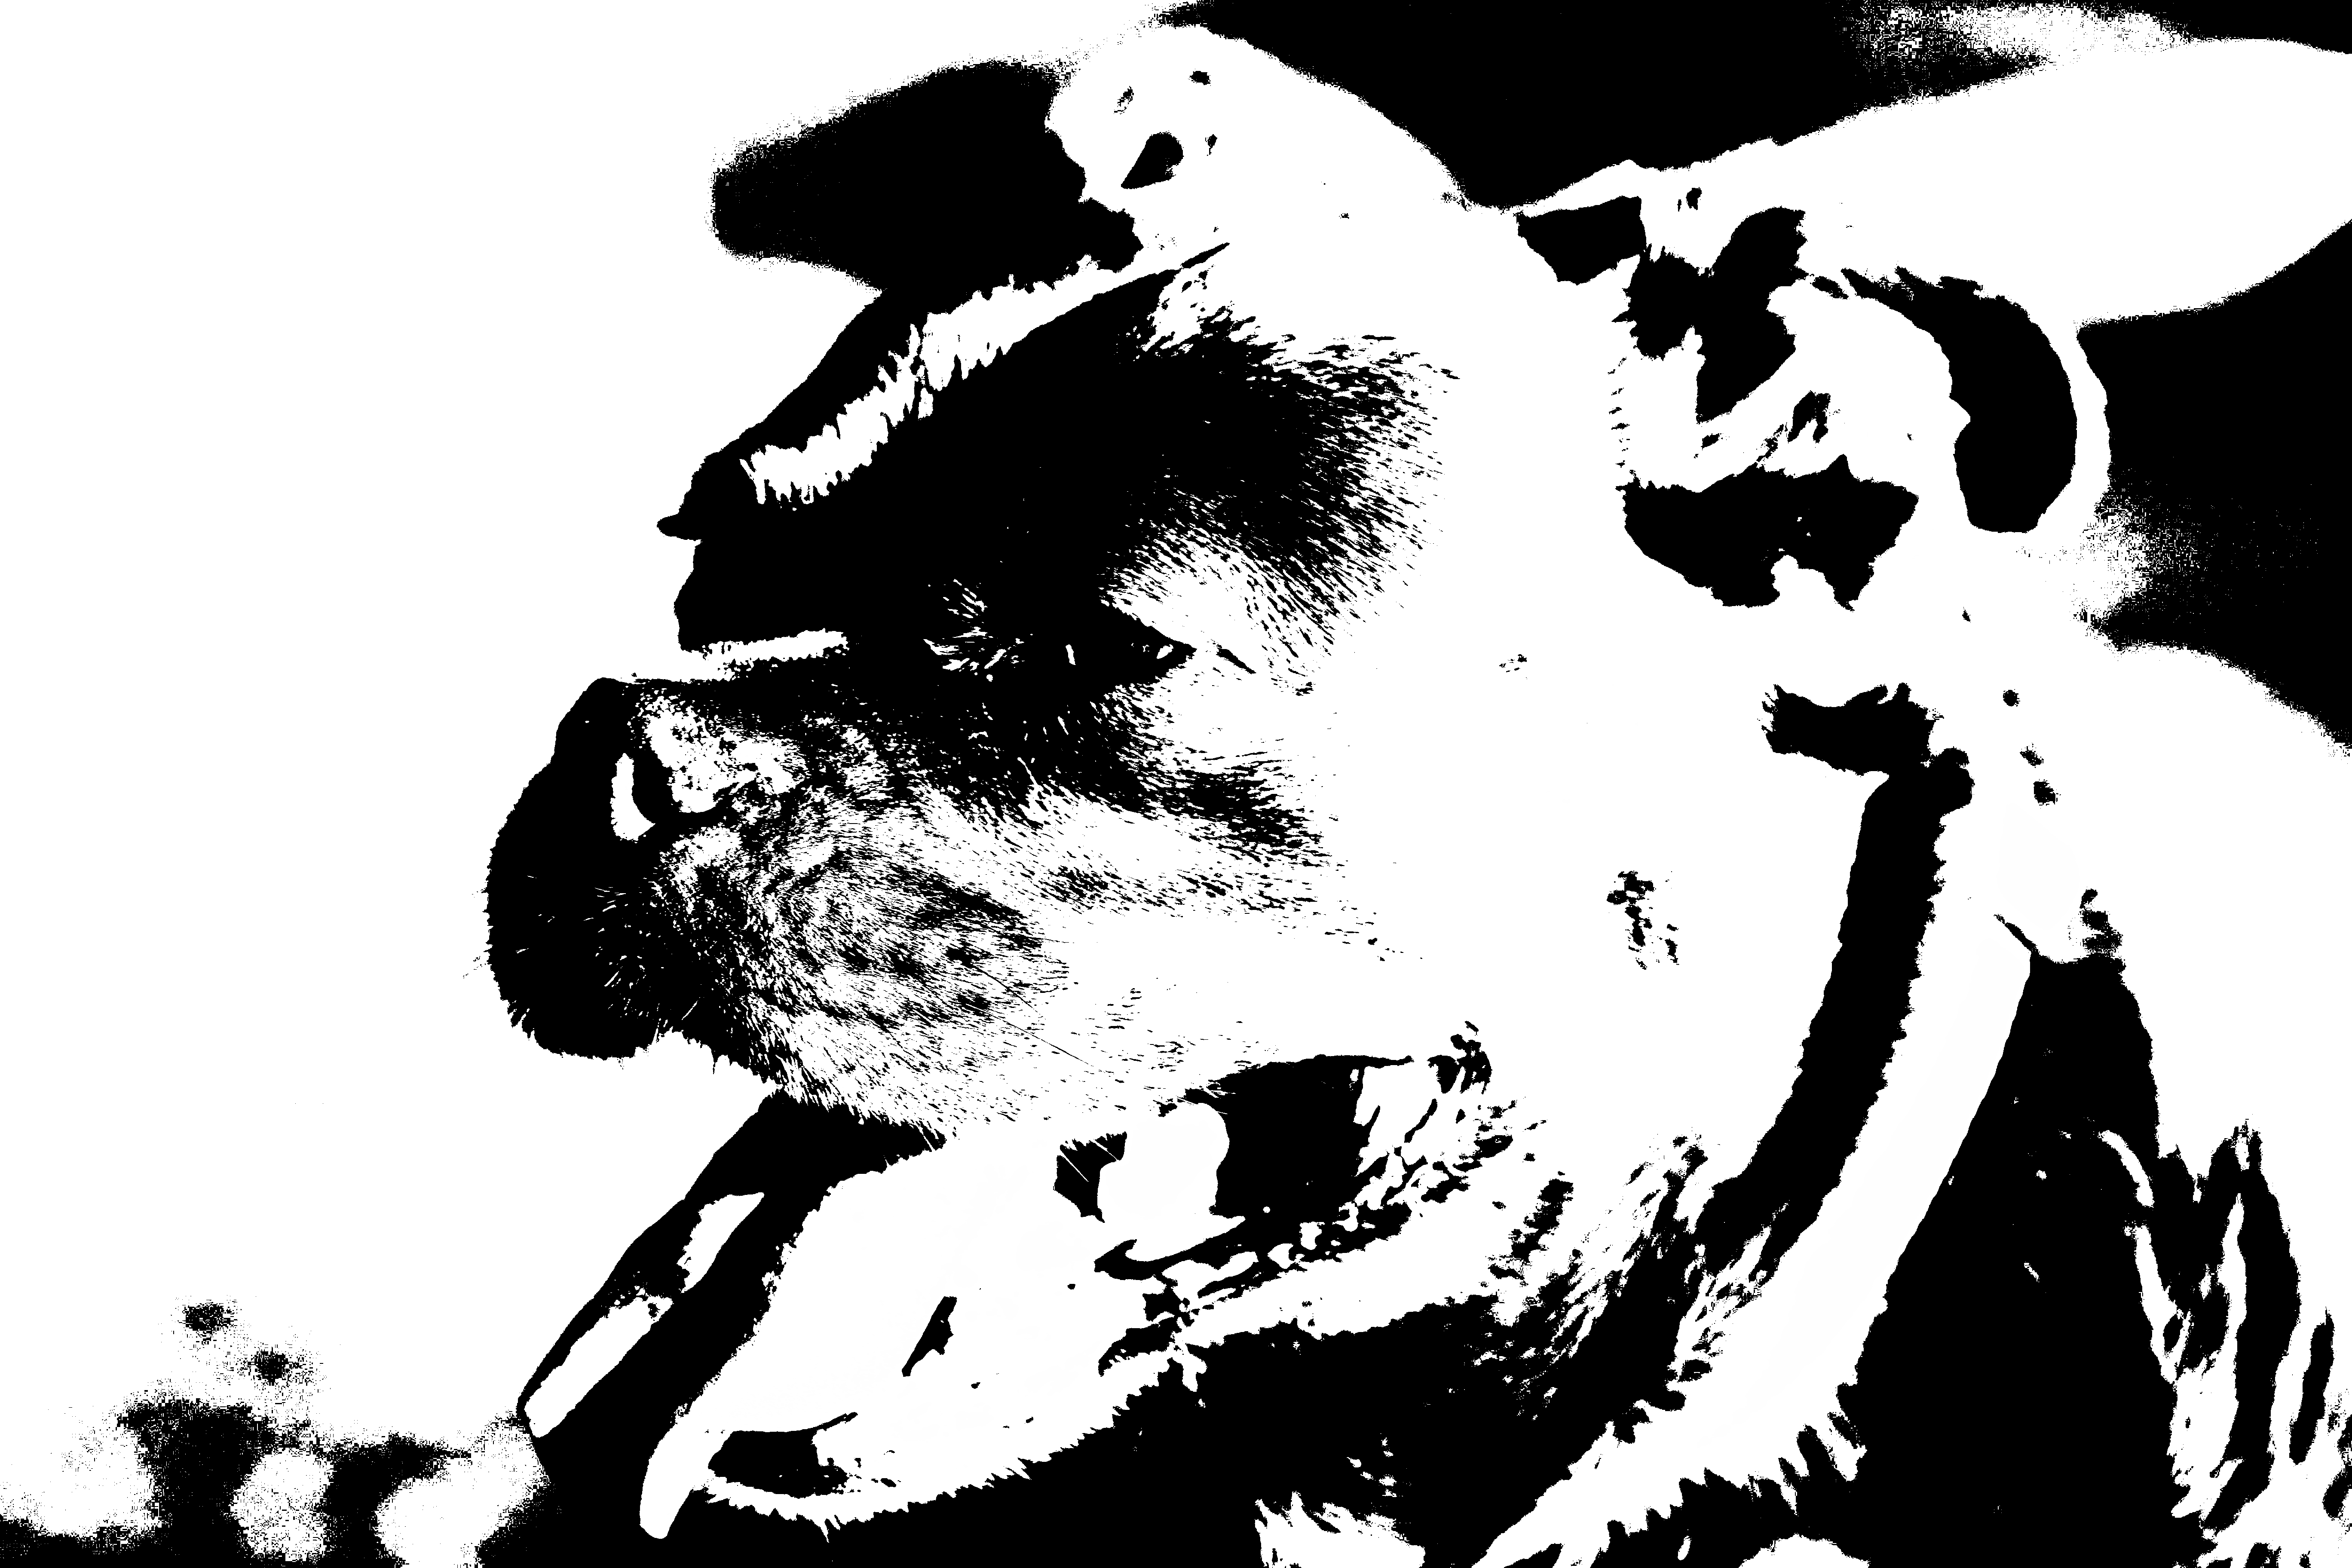
\includegraphics[width=0.8\linewidth]{modified_tsmo_image.png}
    \caption{The image produced by the new peaks multi-threshold Otsu's method  }
    \label{fig:new}
\end{figure}



\begin{figure}[h!]
    \centering
    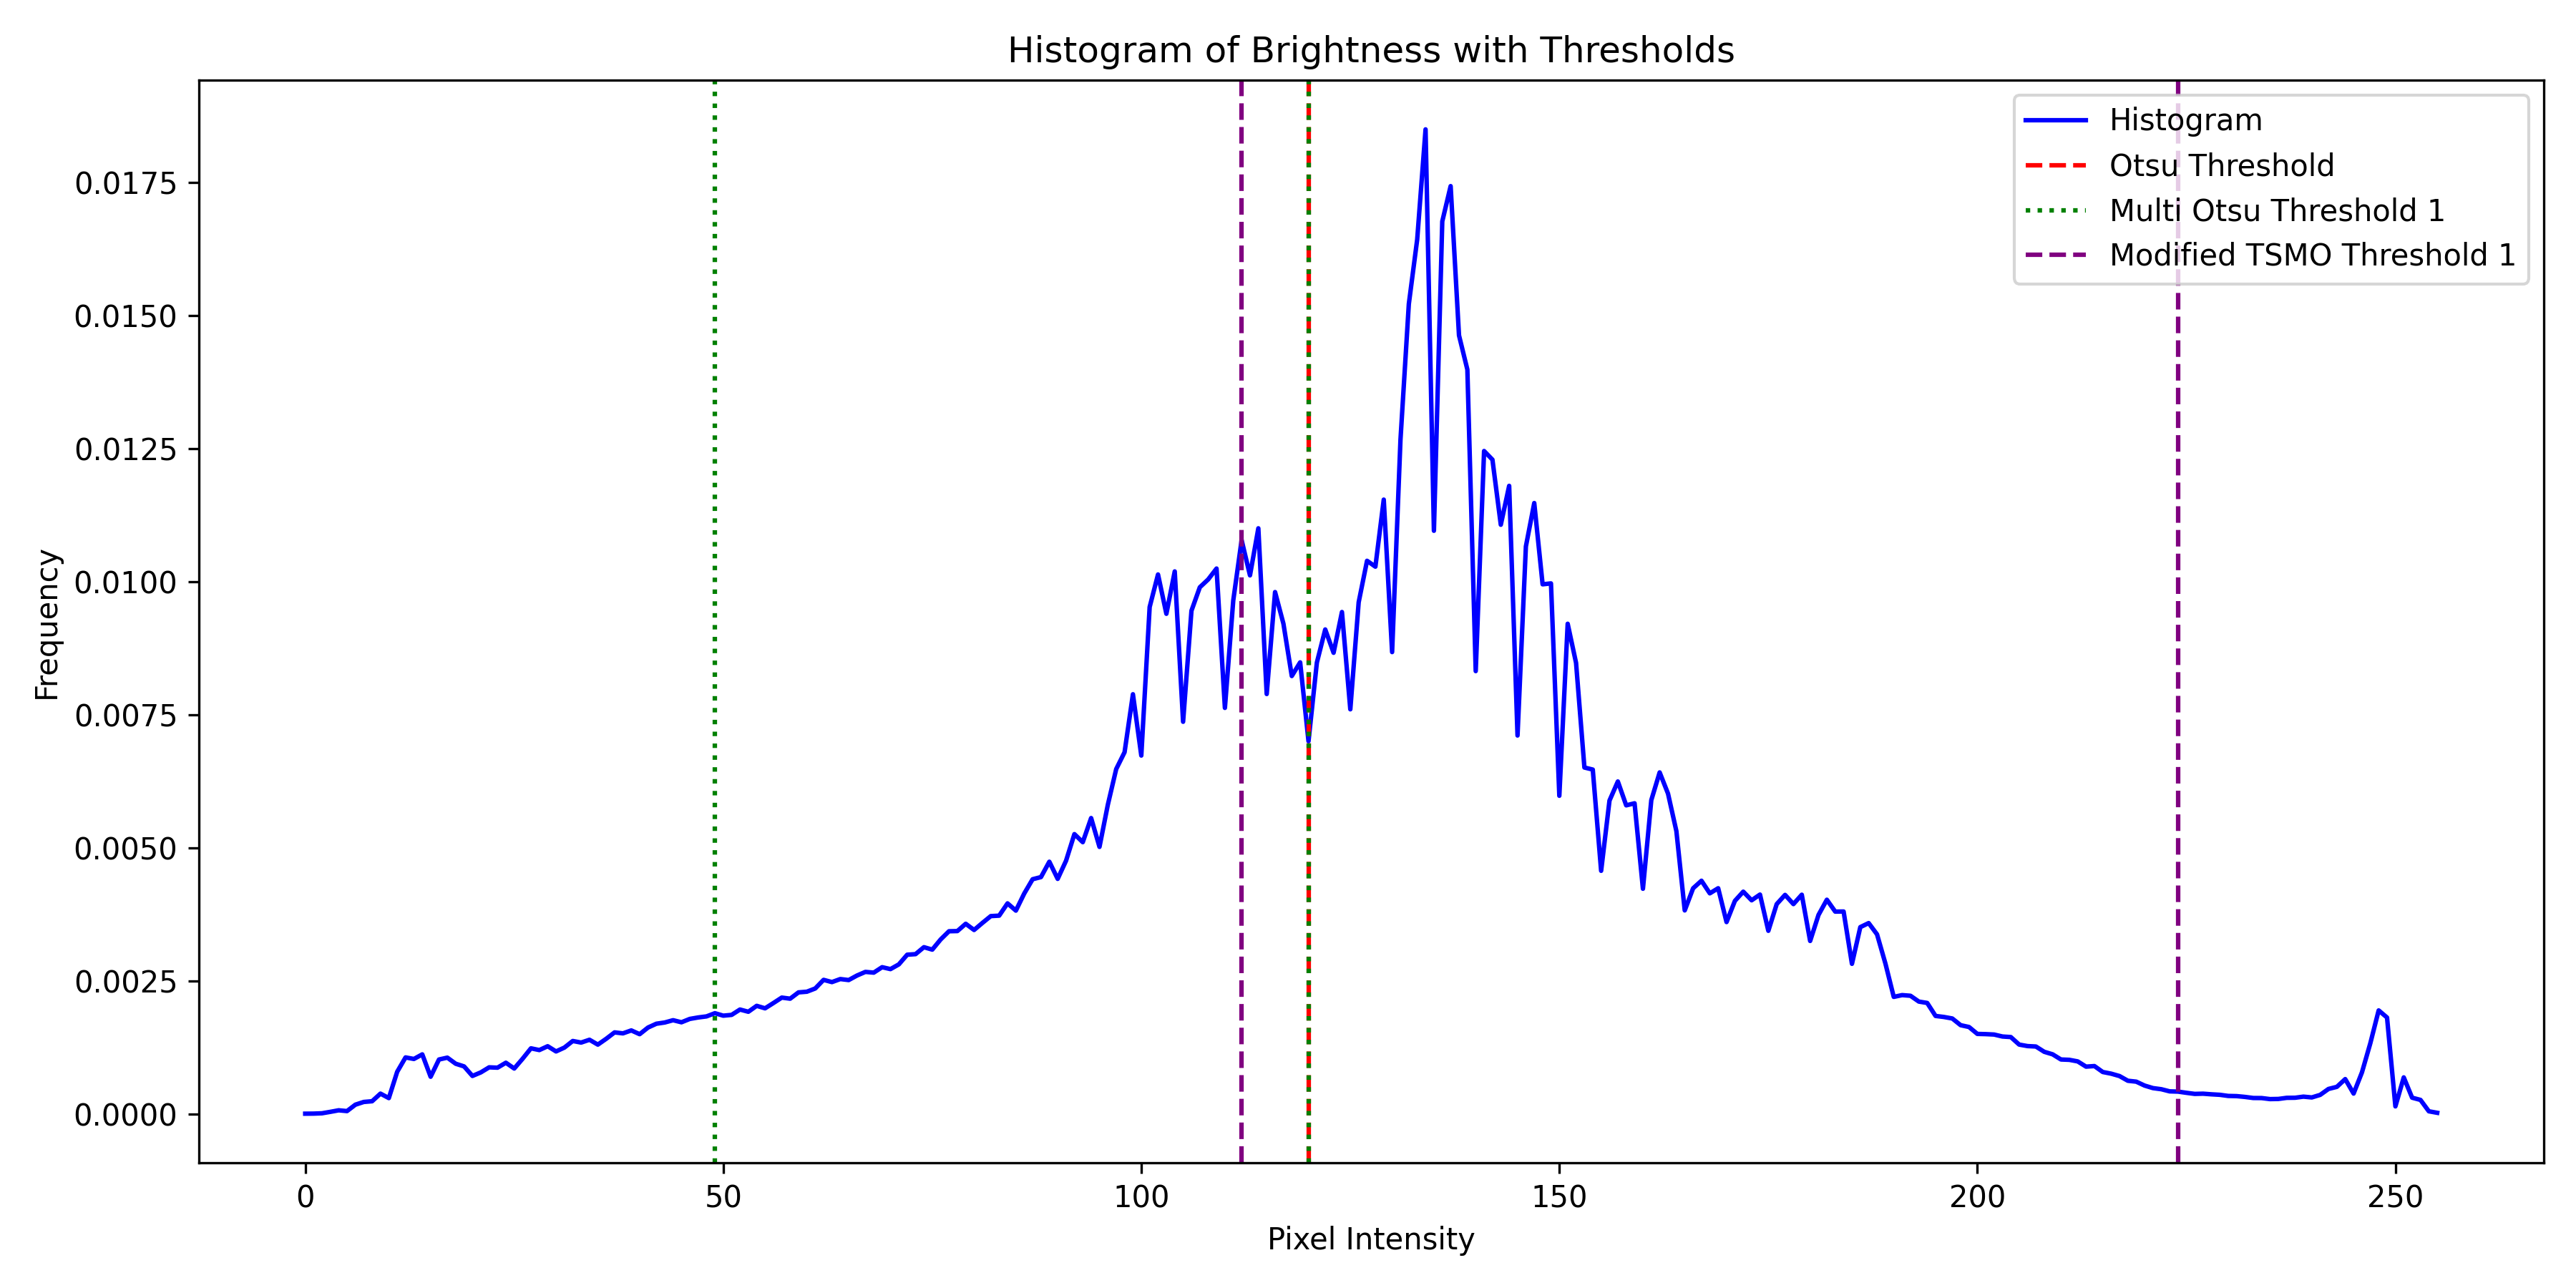
\includegraphics[width=.8\linewidth]{thresholding_result.png}
    \caption{This is the threshold diagram based on the pixel intensity. The dashed green lines are the thresholds for multi-threshold Otsu's method, the red dotted line is the threshold for single-threshold Otsu's method, and the dashed purple lines are the thresholds for the peaks multi-threshold valleys method }
    \label{fig:new}
\end{figure}
\section{Conclusion}
The single-threshold Otsu's method, and multi-threshold Valleys method preformed similarly, which I thought that the new method would preform a lot better. Furthermore, surprisingly, the multi-threshold Otsu's method preformed the worse out of the two methods. However, ultimately the new valleys approach seemed the separate the dog and the background better than all of the methods.

{\small
\bibliographystyle{ieee_fullname}
\bibliography{egbib}

}
\end{document}
